
% =====================================================================
\chapter{Requirements Analysis}
% =====================================================================

\vspace{0.5cm}

\section{Functional requirements}
The functional requirements, grouped by actor, describe what the system must
provide. The last column reports the Priority.

\begingroup
\small
\setlength{\LTpre}{4pt}\setlength{\LTpost}{6pt}

\reqgroup{Common functions}

\begin{longtable}{>{\bfseries}p{1.35cm}>{\raggedright\arraybackslash}p{\dimexpr\linewidth-2.95cm-6\tabcolsep\relax}>{\centering\arraybackslash}p{1.6cm}}
\toprule
\rowcolor{accent}\tablehead{ID} & \tablehead{Requirement} & \tablehead{Priority}\\
\midrule\endhead
\reqrow{RF01}{The system shall authenticate every user before any operation.}{M}
\rowcolor{softgrey}
\reqrow{RF02}{The system shall assign each account a role (patient, doctor, manager) and enable only the functions and the views of that role.}{M}
\bottomrule
\end{longtable}

\reqgroup{Patient}

\begin{longtable}{>{\bfseries}p{1.35cm}>{\raggedright\arraybackslash}p{\dimexpr\linewidth-2.95cm-6\tabcolsep\relax}>{\centering\arraybackslash}p{1.6cm}}
\toprule
\rowcolor{accent}\tablehead{ID} & \tablehead{Requirement} & \tablehead{Priority}\\
\midrule\endhead
\reqrow{RF03}{The patient shall declare the amount of carbohydrates (in grams) they intend to eat. The time of entry is recorded automatically.}{M}
\rowcolor{softgrey}
\reqrow{RF04}{The system shall automatically acquire the glucose level of the patient every 5 minutes through the CGM sensor (simulated via dataset replay).}{M}
\reqrow{RF05}{The system shall predict the patient's glucose level 30 minutes ahead, based on the recent CGM glucose history, meal carbohydrates and device inputs.}{M}
\rowcolor{softgrey}
\reqrow{RF06}{The system shall communicate to the patient one of the possible outcomes: \emph{regular}, the patient may proceed; \emph{carbohydrates above the diet} but glucose within the acceptable range, the patient may proceed but receives a warning; \emph{risk of hyperglycemia}; \emph{risk of hypoglycemia}.}{M}
\reqrow{RF07}{In case of predicted hyperglycemia or hypoglycemia, the system shall record a flag visible to the doctor in charge of the patient, without instant notification.}{M}
\rowcolor{softgrey}
\reqrow{RF08}{The patient shall be able to consult the history of their meals, glucose values and outcomes.}{C}
\bottomrule
\end{longtable}

\newpage

\reqgroup{Doctor}
\begin{longtable}{>{\bfseries}p{1.35cm}>{\raggedright\arraybackslash}p{\dimexpr\linewidth-2.95cm-6\tabcolsep\relax}>{\centering\arraybackslash}p{1.6cm}}
\toprule
\rowcolor{accent}\tablehead{ID} & \tablehead{Requirement} & \tablehead{Priority}\\
\midrule\endhead
\reqrow{RF09}{The doctor shall see in a table only the patients assigned to them, with the status of each patient and the flags received.}{M}
\rowcolor{softgrey}
\reqrow{RF10}{Once a patient is selected, the doctor shall see the trend over time: declared carbohydrates, measured glucose and 30-minute predictions.}{M}
\reqrow{RF11}{The system shall show the comparison between predicted and measured glucose and highlight the deviations.}{M}
\rowcolor{softgrey}
\reqrow{RF12}{The system shall indicate the trends, such as isolated episodes, frequent intake of carbohydrates above or below the diet, and recurring over- or underestimation errors of the model.}{S}
\reqrow{RF13}{The doctor shall be able to register a new patient and set their initial diet.}{M}
\rowcolor{softgrey}
\reqrow{RF14}{The doctor shall be able to update the prescribed diet of a patient.}{C}
\reqrow{RF15}{The doctor shall be able to record an intervention (reminder or diet change) and indicate its cause (model error or patient behavior).}{M}
\bottomrule
\end{longtable}

\reqgroup{Center manager}
\begin{longtable}{>{\bfseries}p{1.35cm}>{\raggedright\arraybackslash}p{\dimexpr\linewidth-2.95cm-6\tabcolsep\relax}>{\centering\arraybackslash}p{1.6cm}}
\toprule
\rowcolor{accent}\tablehead{ID} & \tablehead{Requirement} & \tablehead{Priority}\\
\midrule\endhead
\reqrow{RF16}{The manager shall have a dashboard with aggregated statistics, without access to the personal data of single patients.}{M}
\rowcolor{softgrey}
\reqrow{RF17}{The dashboard shall show the statistical interactions between doctors and patients.}{M}
\reqrow{RF18}{The dashboard shall show the performance of the service, such as response times, availability and compliance with the service level agreement.}{M}
\bottomrule
\end{longtable}

\reqgroup{Model and data}
\begin{longtable}{>{\bfseries}p{1.35cm}>{\raggedright\arraybackslash}p{\dimexpr\linewidth-2.95cm-6\tabcolsep\relax}>{\centering\arraybackslash}p{1.6cm}}
\toprule
\rowcolor{accent}\tablehead{ID} & \tablehead{Requirement} & \tablehead{Priority}\\
\midrule\endhead
\reqrow{RF19}{The system shall periodically update the prediction model, training it offline on the collected data, and make the new version available for predictions.}{M}
\rowcolor{softgrey}
\reqrow{RF20}{The system shall use a unified global model capable of serving all patients immediately (including newly registered patients), dynamically adapting to individual metabolic trends through the recent sliding-window time series without requiring per-patient retraining.}{M}
\reqrow{RF21}{The system shall detect how regularly each patient declares meals.}{C}
\bottomrule
\end{longtable}
\endgroup

\section{Non-functional requirements}
The ten non-functional requirements, grouped into four areas, derive from the
Service Level Agreement of the project and from the health nature of the data.

\begin{table}[H]
\centering
\caption{Performances that must be guaranteed according to the Service Level Agreement.}
\label{tab:sla}
\small
\begin{tabular}{p{4.6cm}p{9.3cm}}
\toprule
\rowcolor{accent}\tablehead{Target} & \tablehead{Value}\\
\midrule
Uptime & From 6:00 to 22:00, 7 days a week (16 hours per day) \\
\rowcolor{softgrey}
Availability & $\geq 99.5\%$ of the uptime (about 4.8 minutes of downtime per day) \\
Reliability & $\geq 99.5\%$ of the uptime \\
\rowcolor{softgrey}
Outage duration & At most 30 minutes, 3 minutes on average \\
Response time & $\leq 1$ second \\
\rowcolor{softgrey}
Customers & About 50\,000 \\
Prediction requests & Up to 5\,000 per minute \\
\rowcolor{softgrey}
Sensor samples & One every 5 minutes per patient \\
\bottomrule
\end{tabular}
\end{table}


\begingroup
\small
\setlength{\LTpre}{4pt}\setlength{\LTpost}{6pt}

\reqgroup{Performance and scalability}
\begin{longtable}{>{\bfseries}p{1.5cm}>{\raggedright\arraybackslash}p{\dimexpr\linewidth-3.1cm-6\tabcolsep\relax}>{\centering\arraybackslash}p{1.6cm}}
\toprule
\rowcolor{accent}\tablehead{ID} & \tablehead{Requirement} & \tablehead{Priority}\\
\midrule\endhead
\reqrow{RNF01}{The response time of a prediction, from the declared meal to the outcome, shall be $\leq 1$ s. If the value is not reachable during testing, additional resources or a revision of the service level agreement, agreed with the client, will be evaluated.}{M}
\rowcolor{softgrey}
\reqrow{RNF02}{The system shall sustain up to 5\,000 prediction requests per minute.}{M}
\reqrow{RNF03}{The system shall serve up to 50\,000 users in total.}{M}
\rowcolor{softgrey}
\reqrow{RNF04}{The system shall sustain the continuous acquisition of glucose samples, with one sample every 5 minutes for each monitored patient. The sizing considers the worst case in which almost all the 50\,000 expected users are patients, that is about 10\,000 writes per minute. It is assumed that glucose is acquired by a sensor with a 5-minute frequency.}{M}
\bottomrule
\end{longtable}

\reqgroup{Availability and reliability}
\begin{longtable}{>{\bfseries}p{1.5cm}>{\raggedright\arraybackslash}p{\dimexpr\linewidth-3.1cm-6\tabcolsep\relax}>{\centering\arraybackslash}p{1.6cm}}
\toprule
\rowcolor{accent}\tablehead{ID} & \tablehead{Requirement} & \tablehead{Priority}\\
\midrule\endhead
\reqrow{RNF05}{The service shall be active every day from 6:00 to 22:00, with availability and reliability $\geq 99.5\%$.}{M}
\rowcolor{softgrey}
\reqrow{RNF06}{Each outage shall last at most 30 minutes, with an average duration of 3 minutes.}{M}
\reqrow{RNF07}{Meals that are not declared or missing samples shall not cause errors: the system still produces an outcome, or reports it as not available.}{S}
\bottomrule
\end{longtable}

\reqgroup{Security and privacy}
\begin{longtable}{>{\bfseries}p{1.5cm}>{\raggedright\arraybackslash}p{\dimexpr\linewidth-3.1cm-6\tabcolsep\relax}>{\centering\arraybackslash}p{1.6cm}}
\toprule
\rowcolor{accent}\tablehead{ID} & \tablehead{Requirement} & \tablehead{Priority}\\
\midrule\endhead
\reqrow{RNF08}{Each user shall access only the data of their role, with a server-side control: a doctor does not read the data of patients who are not assigned, and the manager does not read personal data.}{M}
\rowcolor{softgrey}
\reqrow{RNF09}{The security measures are defined according to the health nature of the processed data. In particular, health data are protected in transit and at rest, and the center manager accesses only aggregated statistics, without the personal data of single patients.}{M}
\bottomrule
\end{longtable}

\reqgroup{Maintainability}
\begin{longtable}{>{\bfseries}p{1.5cm}>{\raggedright\arraybackslash}p{\dimexpr\linewidth-3.1cm-6\tabcolsep\relax}>{\centering\arraybackslash}p{1.6cm}}
\toprule
\rowcolor{accent}\tablehead{ID} & \tablehead{Requirement} & \tablehead{Priority}\\
\midrule\endhead
\reqrow{RNF10}{The model can be replaced or retrained without stopping the service.}{S}
\bottomrule
\end{longtable}
\endgroup

% =====================================================================
\section{Use cases}
% =====================================================================
The system offers eight use cases for the three actors, and all of them must include
UC01, as shown in the use case diagram. The prediction, the recording of the flag and the comparison with the
value measured by the sensor are internal steps of the system and are not
use cases.

\begin{table}[H]
\centering
\caption{Use cases and the requirements they cover.}
\label{tab:usecases}
\small
\begin{tabular}{>{\bfseries}p{1.2cm}p{5.9cm}p{2.3cm}p{4.5cm}}
\toprule
\rowcolor{accent}\tablehead{ID} & \tablehead{Use case} & \tablehead{Actor} & \tablehead{Requirements}\\

\midrule
UC01 & Log in & All & RF01, RF02, RNF08\\
\rowcolor{softgrey}
UC02 & Declare a meal and receive the outcome & Patient & RF03, RF04, RF05, RF06, RF07, RF20, RNF01\\
UC03 & View own history & Patient & RF08\\
\rowcolor{softgrey}
UC04 & View the list of patients & Doctor & RF09, RNF08\\
UC05 & Analyze the trend of a patient & Doctor & RF10, RF11, RF12, RF21\\
\rowcolor{softgrey}
UC06 & Record an intervention & Doctor & RF14, RF15\\
UC07 & Register a new patient & Doctor & RF13, RF20\\
\rowcolor{softgrey}
UC08 & View the service dashboard & Manager & RF16, RF17, RF18, RNF09\\
\bottomrule
\end{tabular}
\end{table}


\subsection{Use Case Diagram}

\begin{figure}[H]
\centering
    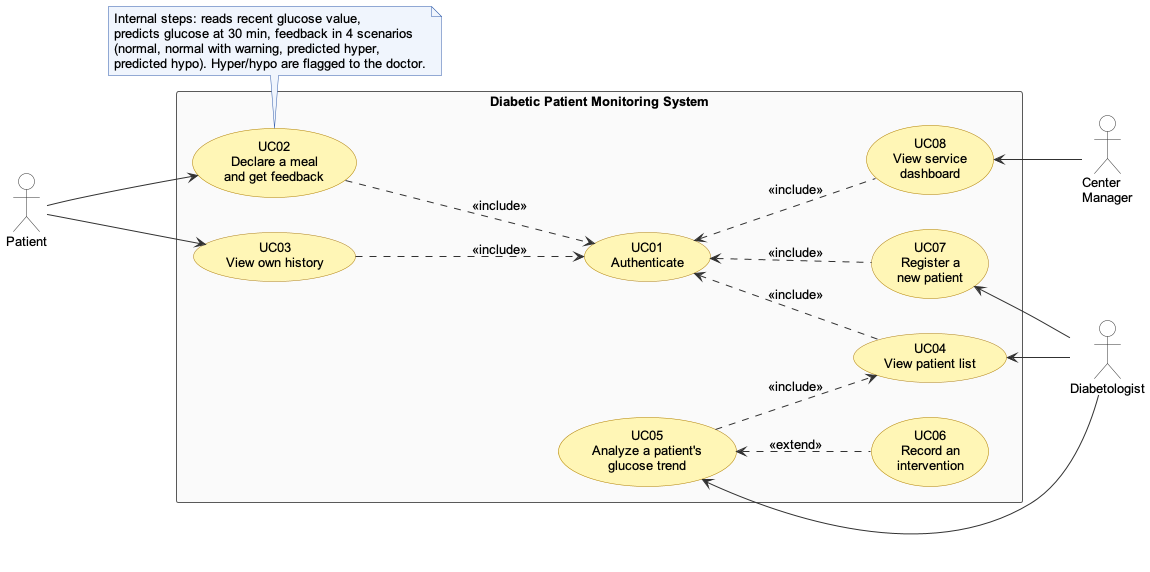
\includegraphics[width=1.0\linewidth]{attach/use_cases_v3.png}
    \caption{Use case diagram illustrating the interactions between patients, diabetologists, and center managers with the system's core functionalities.}
    \label{fig:placeholder}
\end{figure}